\chapter{HRIO Shallow Convection Scheme}
\minitoc

%{\em by R. Honnert}

\section{Introduction}

The grey zone of turbulence is defined by Wyngaard (2004) as the scales on the order of the energy-containing turbulence scale. At these resolutions, the turbulence structures are neither entirely subgrid scale (as in global and mesoscale models) nor largely resolved (as in large-eddy simulations (LES)). Honnert et al. (2011) used LES coarse-graining to produce similarity functions linking the subgrid or resolved part of the turbulent fluxes and the horizontal resolution of the model out of the height of the thermals. They indicated that the grey zone exists from resolutions smaller than two times the boundary-layer height in convective boundary layers (CBL). Regional models are now approaching the sub-kilometic scales and Honnert et al. (2011) showed that neither unidirectional (1D) non-local mesoscale boundary-layer (BL) turbulence scheme nor isotropic (3D) LES schemes are appropriate at these scales. That is why the turbulence schemes have to be adapted to the grey zone of turbulence. 

Boutle et al. (2014) blended a 3D-Smagorinsky with a 1D non-local BL scheme with the help of the similarity functions proposed by Honnert et al. (2011). Ito et al. (2015) extended the Mellor and Yamada scheme by modifiing the length scales using statistics obtained from LES coarse-graining. Shin and Hong (2015) quantified the local and non-local turbulence at scales in the grey zone to adjust the vertical profiles resulting from their non-local K-gradient scheme.  

These adaptations stongly depend on the schemes which are currently used at mesoscale or LES. At M\'et\'eo-France, the turbulence in the atmospheric BL is represented by an eddy-diffusivity/mass-flux  parametrization (EDMF - Hourdin et al. (2002), Soares et al. (2004)). The updraughts are represented by the mass-flux scheme which starts at the ground (hereafter PM09 - Pergaud et~al., 2009 ) and represents the shallow convection, while the rest of the turbulence is represented by a K-gradient scheme (hereafter CBR - Cuxart et~al., 2000)). Both parts of this scheme are being modified to adapt M\'et\'eo-France models to the grey zone of turbulence.   
In this article, modifications of PM09 are presented in the second section as well as preliminary results in the third section. As perspective, the "true" CBR mixing lengths in the grey zone are presented.

\section{Description of the scheme}

As many mass-flux schemes, PM09 is based on several assumptions which are valid at large scales. It assumes in particular that the thermal surface is small, the resolved vertical velocity is zero, and the thermal field is quasi-stationnary. 

Honnert at al. (2016) determined the characteristics of the non-local turbulence (BL thermals) in the grey zone by means of a conditional sampling. Figure~\ref{f01} shows a $16$-km long horizontal cross-section of an LES. The thermals (in white) and the part of the thermals which impact the subgrid mass-flux scheme at $1$-km resolution (in black) have been determined by the conditional sampling of Honnert at al. (2016). The environment of the structures is in red. Figure~\ref{f01} shows that at $16$-km resolution, PM09's assumptions are valid : the thermal surface is small, the resolved vertical velocity is zero, as the grid-cell contains both the updraughts and the compensatory subsidence, and the thermal field is quasi-stationnary. However, in the grey-zone, they are not verified. Indeed, as seen on the $1$-km zoom of Fig.~\ref{f01}, the thermal surface (in black) may be large, the resolved vertical velocity is not zero, as one thermal can fill the grid-cell, and the thermal field is probably not quasi-stationnary.   
\begin{figure}[h!]
	\centering
	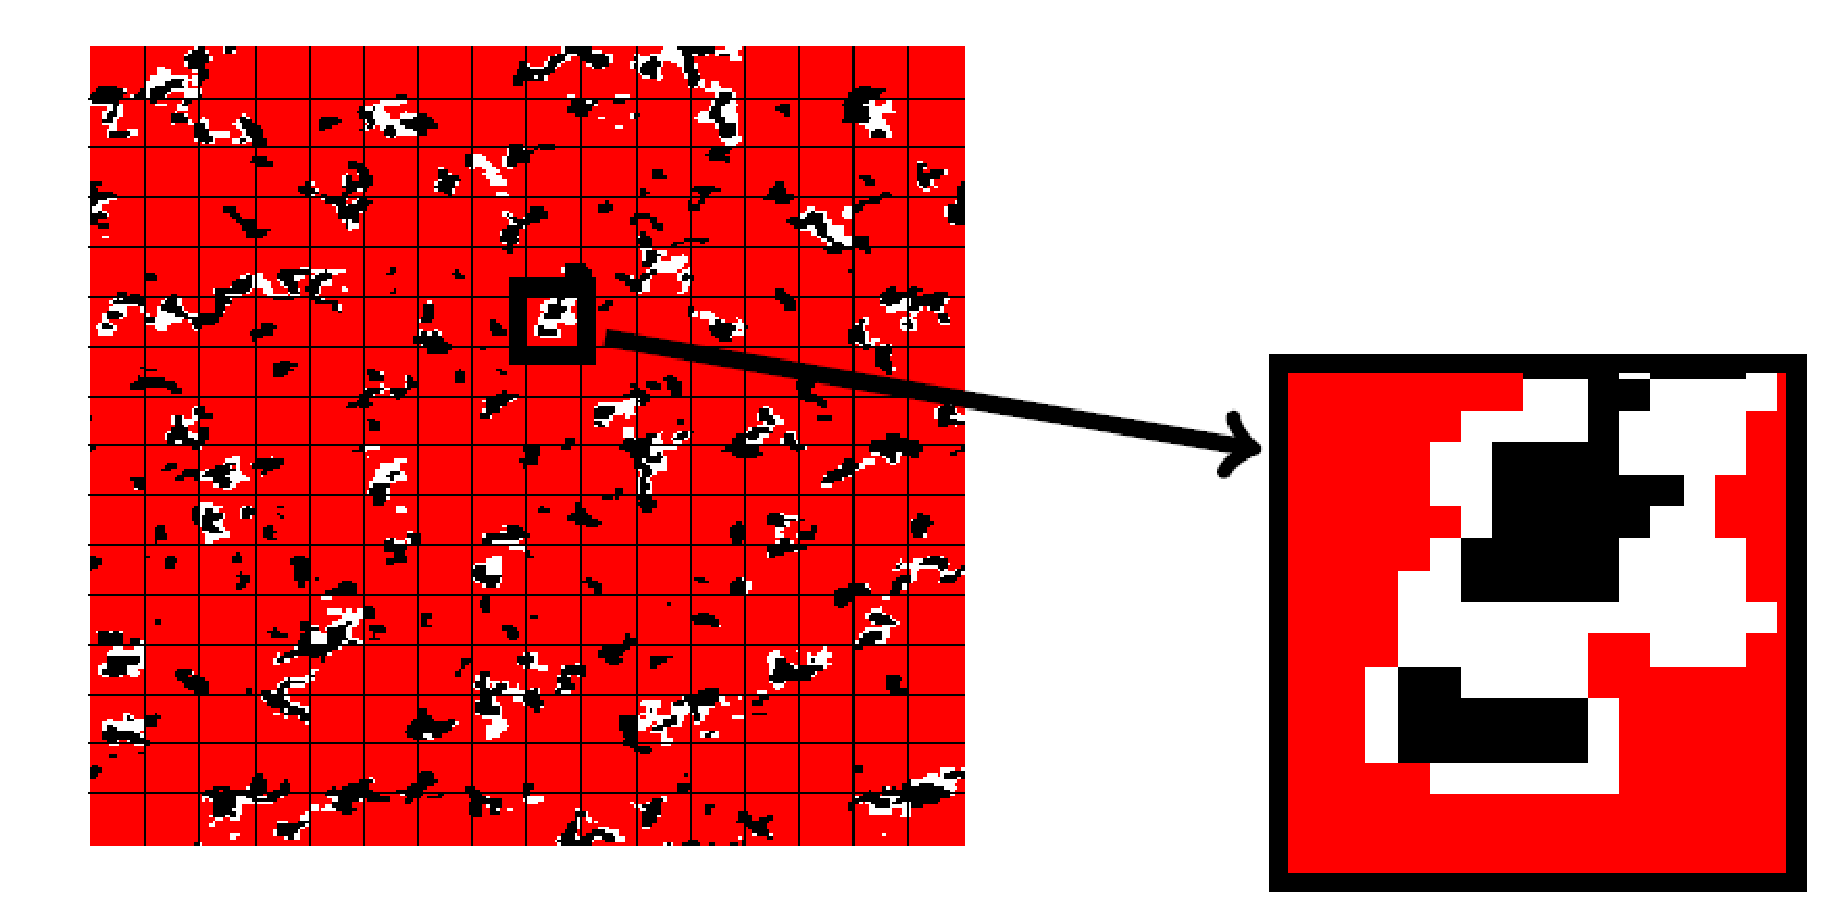
\includegraphics[width=0.8\textwidth]{EPS/f01}
	\caption{\label{f01}$16$-km long horizontal cross-section of an LES (IHOP case , 1400 LT, $500$-m altitude) and $1$-km long zoom. The thermal fraction is in white, the core of the thermals (strong vertical velocity) is in black and the environment is in red. See Honnert et al. (2016)}
\end{figure}

However, mass-flux schemes can be developed without the three assumptions presented before. The initial schemes (PM09, Rio et al. 2009) describe the behaviour of parameters of one unique thermal in the mesh (the vertical velocity $w_u$, the mass-flux $M_u$, the total potential temperature ${\theta_l}_u$, the thermal surface area $\alpha$, the buoyancy inside the thermal $B_u$ and the pressure and the entrainment ($\epsilon$)/ detrainment ($\delta$) lateral closure). $a_1$ and $b_1$ are constant. 
Eq.~(1-4) show the modifications (in red) of PM09. The non-negligible resolved vertical velocity ($\overline{w}^{\Delta x}$) is added in Eq.~(1,3-4). The thermal surface is not negligible and appears at the denominator in Eq.~(3-4). The surface triggering of the mass-flux (${M_u}_{z=0}$, Eq.~(5)) depends on the resolution.  

\begin{eqnarray}
	M_u&=&\rho\alpha(w_u\color{red}{-\overline{w}^{\Delta x}}\color{black}{)}\\
	\frac{1}{M_u}\frac{\partial M_u}{\partial z}&=&\epsilon-\delta\\
	\frac{\partial {\theta_l}_u}{\partial z}&=&-\frac{\color{red}{\epsilon}}{\color{red}{1-\alpha}}({\theta_l}_u -\overline{\theta_l}^{\Delta x})\\
	\frac{1}{2}\frac{\partial (w_u\color{red}{-\overline{w}^{\Delta x}\color{black}{)}^2}\color{black}{)}}{\partial z}&=&a_1B_u-b_1\frac{\color{red}{\epsilon}}{\color{red}{1-\alpha}}(w_u\color{red}{-\overline{w}^{\Delta x}}\color{black}{)^2}\\
\end{eqnarray}

Then, the finer the resolution or the smaller the BL height, the smaller the subgrid turbulent flux. The scheme produces less subgrid turbulence. Consequently, resolved BL thermals are created.

\section{Initialisation of Mass-Flux scheme}


he triggering controls the activation of the mass-flux scheme at the surface while the closure controls its intensity. Often the boundary-layer mass-flux scheme triggers as soon as the surface sensible heat flux is positive while the intensity of the mass-flux at the ground is proportional to the convective velocity scale (see Pergaud et~al.,2009). 

Firstly, concerning the closure, Figure~\ref{trigDavid}a shows the subgrid mass-flux normalized by the convective velocity scale as a function of the normalized resolution in the IHOP case at $1200$ LT and the ARM case at $1400$ LT in the middle of the boundary layer. The mass-flux normalized by the convective velocity scale in both the IHOP and ARM cases is dependent on the resolution normalized by the height of the thermals : it is constant at mesoscales and larger than in LES. Here the mass flux is computed in the middle of the CBL. It cannot be diagnosed directly at the ground where there is no really thermal formed yet and where the turbulent is more strongly dependent on the subgrid turbulence scheme. The normalized mass flux as a function of the normalized resolution has the same shape at all altitudes in the boundary layer (not shown). Therefore, here we propose to make the constant of proportionality between the mass-flux at the ground and the convective velocity scale (computed at ground level for the whole domain, $w*$) dependent on the resolution by this function :

\begin{equation}
	\sigma(\frac{M_u}{w_*})=tanh(C\times\sqrt(\Delta x \times \Delta y)/L_{up})
\label{eq:MuHect}
\end{equation}
In the magenta fit plotted in Fig.~\ref{trigDavid}a, $C=1.83$. We propose to use this function in the parametrization in order to make it scale-aware.

Moreover, the subgrid mass-flux variability is larger in the grey zone than in the LES and at mesoscales. This is visible in Fig.~\ref{trigDavid}b which shows the standard deviation of the mass-flux normalized by the convective velocity scale ($\sigma(\frac{M_u}{w*})$) as a function of the normalized resolution in the IHOP case at $1200$~LT and the ARM case at $1400$~LT in the middle of the CBL. The large variability in the grey zone is also visible on the buoyancy and the entrainment (cf.~Honnert et al., 2016) and it is consistent with Dorrestijn et al. (2013) which showed that the heat flux variability is larger in the grey zone. The fit of the data of Fig.~\ref{trigDavid}b is:

Concequently, the closure of the mass-flux scheme of Pergaud et~al. (2009) at hectometric scales depend on the model resolution following Eq.~\ref{eq:MuHect}.

\section{References}

\noindent \por
Boutle, I. A., Eyre, J. E. J., and Lock, A. P., 2014:
Seamless stratocumulus simulation across the turbulent grey zone. 
{\it Mon. Wea. Rev.}, {\bf 42}, 1655--1668. 

\noindent \por
Cuxart, J., P. Bougeault, and J.-L. Redelsperger, 2000:
A turbulence scheme allowing for mesoscale and large-eddy simulations.
{\it Quart. J. Roy. Meteor. Soc.}, {\bf 126,} 1--30.

\noindent \por
Dorrestijn J, Crommelin DT, Siebesma AP and Jonker HJJ, 2013:
Stochastic convection parametrization estimated from high-resolution model data.  27:133--148
{\it Theor Comput Fluid Dyn}, {\bf 27}, 133--148.

\noindent \por
Honnert, R., Masson, V., and Couvreux, F., 2011:
A diagnostic for evaluating the representation of turbulence in atmospheric models at the kilometric scale.  
{\it J. Atmos. Sci.}, {\bf 68(12)}, 3112--3131.

\noindent \por
Honnert, R., Couvreux, F., Masson, V., and David Lancz, 2016 :
Sampling the Structure of Convective Turbulence and Implications for Grey-Zone Parametrizations
{\it Bound. Layer. Meteor.}, {\bf 160}, 133.

\noindent \por
Hourdin, F., F. Couvreux, and L. Menut, 2002:
Parameterization of the Dry Convective Boundary Layer Based on a Mass Flux Representation of Thermals.
{\it J. Atmos. Sci.}, {\bf 59}, 1105--1122.

\noindent \por
Ito, J., Niino, H., Nakanishi, M., and Moeng, C. H., 2015:
An extension of the Mellor–Yamada model to the terra incognita zone for dry convective mixed layers in the free convection regime.
{\it Bound. Layer. Meteor.}, {\bf 157(1)}, 23--43.

\noindent \por
Pergaud, J., V. Masson, S. Malardel, and F. Couvreux, 2009:
A Parameterization of Dry
  Thermals and Shallow Cumuli for Mesoscale Numerical Weather Prediction.
{\it Bound. Layer. Meteor.}, {\bf 132}, 83--106.

\noindent \por
Rio, C., F. Hourdin, J. Y. Grandpeix, and J. P. Lafore, 2009:
Shifting the diurnal cycle of parameterized deep convection over land.
{\it Geophysical Research Letters.}, {\bf 36}, 7.

\noindent \por
Shin, H., and Hong, S., 2013 : 
Analysis on resolved and parametrized vertical transports in the convective boundary layers at the gray-zone resolution. 
{\it J. Atmos. Sci.}, {\bf 70}, 3248--3261.

\noindent \por
Soares, P. M. M., P. M. A. Miranda, A. P. Siebesma, and J. Teixeira, 2004:
An Eddy-Diffusivity/Mass-Flux parameterization for dry and shallow cumulus
  convection.
{\it Quart. J. Roy. Meteor. Soc.}, {\bf 130}, 3055--3079.

\noindent \por
Wyngaard JC, 2004 : 
Toward numerical modelling in the ‘Terra Incognita’. J Atmos Sci 61:1816–1826
{\it J. Atmos. Sci.}, {\bf 61}, 1816--1826.
